\documentclass[18pt]{beamer}

%% SLIDE FORMAT

% use 'beamerthemekit' for standard 4:3 ratio
% for widescreen slides (16:9), use 'beamerthemekitwide'

%\usepackage{templates/beamerthemekit}
\usepackage{templates/beamerthemekitwide}
\usepackage{amsmath}
\usepackage{amssymb}
\usepackage[ngerman]{babel}
\usepackage{graphicx}
\usepackage{color}
\usepackage[utf8]{inputenc}
\usepackage[english]{babel}
\usepackage{minted}

%% TITLE PICTURE

% if a custom picture is to be used on the title page, copy it into the 'logos'
% directory, in the line below, replace 'mypicture' with the 
% filename (without extension) and uncomment the following line
% (picture proportions: 63 : 20 for standard, 169 : 40 for wide
% *.eps format if you use latex+dvips+ps2pdf, 
% *.jpg/*.png/*.pdf if you use pdflatex)

%\titleimage{board}

%% TITLE LOGO

% for a custom logo on the front page, copy your file into the 'logos'
% directory, insert the filename in the line below and uncomment it

\titlelogo{blank}

% (*.eps format if you use latex+dvips+ps2pdf,
% *.jpg/*.png/*.pdf if you use pdflatex)

%% TikZ INTEGRATION

% use these packages for PCM symbols and UML classes
% \usepackage{templates/tikzkit}
% \usepackage{templates/tikzuml}

% the presentation starts here

\title[Prologadapter für Java]{Prologadapter für Java}
\subtitle{Betreut von Stephan Seifermann}
\author{Johannes Werner}

\institute{Fakultaet für Informatik}

% Bibliography

\usepackage[citestyle=authoryear,bibstyle=numeric,hyperref,backend=biber]{biblatex}
\addbibresource{templates/example.bib}
\bibhang1em
{\renewcommand{\arraystretch}{1.3}
\begin{document}

% change the following line to "ngerman" for German style date and logos
\selectlanguage{ngerman}

%title page
\begin{frame}
\titlepage
\end{frame}

%table of contents
\begin{frame}{Gliederung}
\tableofcontents
\end{frame}

\section{Motivation}
\begin{frame}{Motivation}
\begin{itemize}
\item Sprachen haben unterschiedliche St"arken
% Python vs C
%
% Mit Python kann man schnell entwickeln, sehr abstrakte Sprache.
% In C kann man rechenintensive Algorithmen auslagern, um die
% Performance zu erh"ohen, oder wenn man platformspezifische
% Funktionalitaet braucht
\item St"arken kombinierbar?
\vspace{0.2cm}
\item Implementierungen einer Sprache haben unterschiedliche St"arken
% Proprietary vs Open source
% Moegliche Lizenzkonflikte vermeiden
% Spezielle Optimierungen implementiert
\item Mehrere Implementierungen nutzbar?
\vspace{0.2cm}
\item \textbf{L"osung:} Adapter einsetzen
\end{itemize}
\begin{figure}[h]
\centering
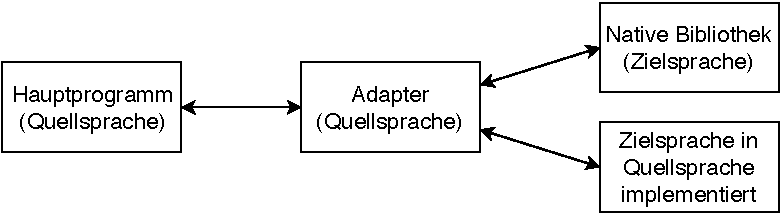
\includegraphics[width=0.9\textwidth]{adapter.pdf}
\end{figure}
\end{frame}

\section{Anforderungen}
\begin{frame}{Anforderungen}
\begin{itemize}
\item \textbf{Kontext:} Adapter soll in Eclipse-Plugin verwendet werden
\vspace{0.3cm}
\item Interpreter m"ussen EPL-kompatible Lizenz haben
% Eclipse Plugins laufen unter der EPL Lizenz, d.h. jede verwendete Software muss EPL
% kompatibel sein
\vspace{0.3cm}
\item Anbindung zu mehreren Interpretern
% Siehe weiter oben. Verschiedene Interpreter haben verschiedene Staerken
\begin{itemize}
\item SWI-Prolog unterst"utzen
% Ist der weitestverbreiteste Interpreter, dementsprechend auch aktiv weiterentwickelt
\item Mindesten ein Interpreter in Java implementiert
% Ein Interpreter soll mit dem Plugin selbst ausgeliefert werden, um
% out-of-the-box funktioieren zu koennen, ohne vom Nutzer erwarten zu muessen,
% ein Interpreter vorinstalliert zu haben
\end{itemize}
\vspace{0.3cm}
\item Java-Objekte als Antwort vom Interpreter
\begin{itemize}
\item Anfrage: String('2+2')
\item Antwort: Integer(4)
\end{itemize}
% Mit den Ergebnissen soll weiter verarbeitet werden und m"ussten sonst
% geparset werden.
\end{itemize}
\end{frame}

\section{Interpreterwahl}
\begin{frame}{Interpreterwahl}
\begin{itemize}
\item \textbf{Kriterien} (* Pflicht)
\begin{itemize}
\item Java-Anbindung*
% Eigene Java-Anbindung waere zu aufwaendig
\item Passende Lizenz*
% siehe oben
\item Paket im Maven-Repository
% Convenience Grund. Vereinfacht den Build-Prozess
\item Java-Implementierung
% siehe oben
\item Zeitpunkt des letzten Releases
% Wenn ein Projekt nicht gewartet wird, kann es sein, dass irgendwann
% kompatibilitaet gebrochen wird
% Bugs werden nicht gefixt
% Moeglicherweise geringer Funktionsumfang
\end{itemize}
\vspace{0.5cm}
\item \textbf{Herausforderung}
\begin{itemize}
\item Es gibt eine Vielzahl an Interpretern
\item Wenige erf"ullen Kriterien
\end{itemize}
\end{itemize}
\end{frame}
\begin{frame}{Interpreterwahl}
\begin{table}[]
\resizebox{\textwidth}{!}{%
\begin{tabular}{r|ccc}
\multicolumn{1}{l|}{} & \textbf{SWI-Prolog} & \textbf{TuProlog} & \textbf{Projog} \\ \hline
Lizenz                & BSD          & LGPL              & Apache 2.0      \\ \hline
Letzter Release       & Juli'19          & Okt'18        & Dez'18      \\ \hline
Maven-Paket           & \checkmark          & \checkmark        & \checkmark      \\ \hline
Java-Implementierung & $\times$            & \checkmark        & \checkmark     
\end{tabular}%
}
\end{table}
\vspace{0.5cm}
\begin{itemize}
\item SWI-Prolog ist der weitestverbreitete und am aktivsten weiterentwickelte Interpreter
\end{itemize}
\end{frame}

\section{Java-Schnittstelle}
\begin{frame}[fragile]{Java-Schnittstelle - Prolog}
Beispiel Prologdatenbank:
\begin{minted}{Prolog}
child_of(Hans, Peter).
child_of(Brigitte, Peter).
\end{minted}
\vspace{1cm}
\textbf{Ziel:} Prolog-Statement in Java ausf"uhren
\begin{minted}{Prolog}
    child_of(Norbert, Peter).
\end{minted}
\end{frame}
\begin{frame}[fragile]{Java-Schnittstelle - Java}
\begin{minted}{Java}
class Human {
    private String name;
    // Getter and Setter are present

    public boolean isChildOf(Human parent) {
        // How to query the prolog database?
        // The query to execute:
        //     child_of(nameOfParent, this.name).
    }	
}
\end{minted}
\end{frame}
\begin{frame}[fragile]{Java-Schnittstelle - SWI-Prolog}
\begin{minted}{Java}
// class Human { ...

public boolean isChildOf(Human parent) {
    // convert(...) can tranform Human into Atom
    Atom parentName = convert(parent);
    Atom childName = convert(this);
    // goal = child_of(parentName, childName)
    Term goal = 
        Util.textParamsToTerm(
            "child_of(?parent, ?child).", 
            parentName, childName);
    Query query = new Query(goal);
    return query.hasMoreSolutions();
}
\end{minted}
\end{frame}
\begin{frame}[fragile]{Java-Schnittstelle - Projog}
\begin{minted}{Java}
// class Human { ...

private Projog engine;

public boolean isChildOf(Human parent) {
    String pName = parent.getName();
    String cName = this.getName();
    QueryResult solution =
        engine.solve("child_of("+pName+","+cName+").");
    return solution.next();
}
\end{minted}
\end{frame}

\section{Prolog4J}
\begin{frame}{Prolog4J}
\begin{itemize}
\item Java-zu-Prolog Adapter
\item MIT-Lizenz (EPL-kompatibel)
\item Unterst"utzte Interpreter
\begin{itemize}
\item SWI-Prolog
\item TuProlog
\item JTrolog
\item JLog
\end{itemize}
\vspace{0.3cm}
\item \textbf{Probleme}
\begin{itemize}
\item Veraltet (Letzter Commit in 2011)
\item Fehlende Funktionali"at
\item Unterst"utzt nicht alle gew"unschten Interpreter
\end{itemize}
\end{itemize}
\end{frame}
\subsection{Architektur}
\begin{frame}[fragile]{Architektur}
\begin{minted}{Java}
// class Human { ...

private Prover p;

public boolean isChildOf(Human parent) {
    Query query = p.query("child_of(?parent, ?child).");
    Solution<?> solution = 
        query.solve(parent, this);
    return solution.isSuccess();
}
\end{minted}
\end{frame}
\begin{frame}{Architektur}
\begin{figure}[h]
\centering
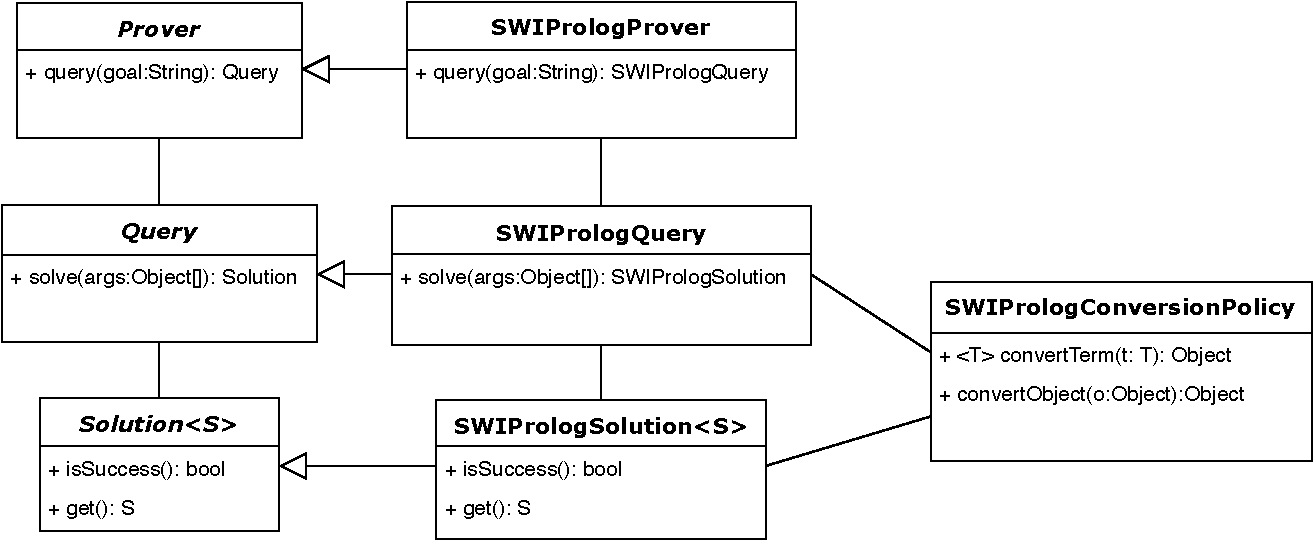
\includegraphics[width=1\textwidth]{prolog4j.pdf}
\end{figure}
\end{frame}



\subsection{Analyse}
\begin{frame}{Analyse}
\begin{itemize}
\item Unterst"utzt nicht alle Interpreter
\begin{itemize}
\item Entfernen nicht ben"otigter Interpreter
\item Projog unterst"utzen
\end{itemize}
\vspace{0.2cm}
\item Veraltet
\begin{itemize}
\item Aktualisieren der POM-Dateien (Maven)
\item Aktualisieren des Codes
\end{itemize}
\vspace{0.2cm}
\item Fehlende Funktionalit"at
\begin{itemize}
\item API erweitern
\item Interpreter-Discovery mit OSGI
\end{itemize}
\end{itemize}
\end{frame}
\begin{frame}[fragile]{Bug in Projog}
\begin{itemize}
\item Neu hinzugef"ugte Regeln f"ur einen Funktor "uberschreiben vorherige Regeln
\begin{itemize}
\item Regeln werden in einer Hashmap gespeichert und "uberschreiben beim Einf"ugen den vorherigen Wert des Funktors
\end{itemize}
\vspace{0.5cm}
\item Folgende Regeln sollen der Datenbank hinzugef"ugt werden
\begin{minted}{Prolog}
human(socrates), human(euklid), human(plato)
\end{minted}
\end{itemize}
\end{frame}
\begin{frame}[fragile]{Bug in Projog}
\begin{itemize}
\item Folgender Code funktioniert
\begin{minted}{Prolog}
addTheory(human(socrates), human(euklid)), human(plato)).
\end{minted}
\vspace{0.5cm}
\item Resultierende Datenbank
\begin{minted}{Prolog}
human(socrates)
human(euklid)
human(plato)
\end{minted}
\end{itemize}
\end{frame}
\begin{frame}[fragile]{Bug in Projog}
\begin{itemize}
\item Folgender Code funktioniert \textbf{nicht}
\begin{minted}{Prolog}
addTheory(human(socrates)).
addTheory(human(euklid)).
addTheory(human(plato)).
\end{minted}
\vspace{0.5cm}
\item Resultierende Datenbank
\begin{minted}{Prolog}
human(plato)
\end{minted}
\end{itemize}
\end{frame}
\begin{frame}{Bug in Projog - L"osung}
\begin{itemize}
\item Eine Liste mit allen Regeln per Funktor wird parallel gehalten
\vspace{0.5cm}
\item Einf"ugen einer Regel:
\begin{enumerate}
\item Einf"ugen der Regel in die eigene Datenbank
\item Einf"ugen der gesamten Datenbank in die Projog-Datenbank
\end{enumerate}
\end{itemize}
\end{frame}
\begin{frame}{Interpreter-Discovery mit OSGI}
\begin{itemize}
\item \textbf{O}pen \textbf{S}ervices \textbf{G}ateway \textbf{i}nitiative
\begin{itemize}
\item Einbinden modularer Services zur Laufzeit
\end{itemize}
\vspace{0.1cm}
\item Einbindung in Laufzeitumgebung von Eclipse
\vspace{0.1cm}
\item Laufzeiterkennung verf"ugbarer Interpreter
\begin{itemize}
\item Kein festes Einprogrammieren n"otig
\item Leichtes Einbinden zuk"unftiger Interpreter
\end{itemize}
\end{itemize}
\end{frame}

\section{Zusammenfassung}
\begin{frame}{Zusammenfassung}
\begin{itemize}
\item Ausf"uhren von Prolog-Befehlen in Java
\item Adapter soll an mehrere Interpreter anbinden
\begin{itemize}
\item SWI-Prolog
\item TuProlog
\item Projog
\end{itemize}
\item Java-Schnittstellen der Interpreter sind unterschiedlich
\item Existierende Bibliothek Prolog4J bietet was wir brauchen
\begin{itemize}
\item Muss modernisiert und erweitert werden
\item Hinzuf"ugen von OSGI Discovery
\end{itemize}
\item M"ogliche Fortsetzung
\begin{itemize}
\item Mehr Interpreter anbinden
\item Ausf"uhrlicher testen
\end{itemize}
\end{itemize}
\end{frame}

% Anhang
\begin{frame}{Projektbezug}
\begin{itemize}
\item Trust 4.0
\begin{itemize}
\item Softwaresystem soll Datenschutz garantieren
\item Architekturmodell wird um Datenflussannotationen erg"anzt
\item Durch Analyse k"onnen Risiken gefunden werden
\end{itemize}
\vspace{0.5cm}
\item Architekturmodell erstellen mit Eclipse-Plugin (\textbf{Java})
\item Datenflussanalyse mittels \textbf{Prolog}
\vspace{0.5cm}
\item[] $\Rightarrow$ \textbf{Java-zu-Prolog Adapter}
\end{itemize}
\end{frame}

\begin{frame}[fragile]{SWI-Prolog Anpassung}
\begin{itemize}
\item Darstellung einer Liste in Standard Prolog
\begin{minted}{Prolog}
'.'([],[])
\end{minted}
\item SWI-Prolog Darstellung
\begin{minted}{Prolog}
'[|]'([],[])
\end{minted}
\vspace{0.5cm}
\item Begr"undung
\begin{minted}{Text}
As of version 7, SWI-Prolog lists can be 
distinguished unambiguously at runtime
from ./2 terms and the atom '[]'
\end{minted}
\end{itemize}
\end{frame}
\begin{frame}{Interpreter-Discovery mit OSGI}
\begin{figure}[h]
\centering
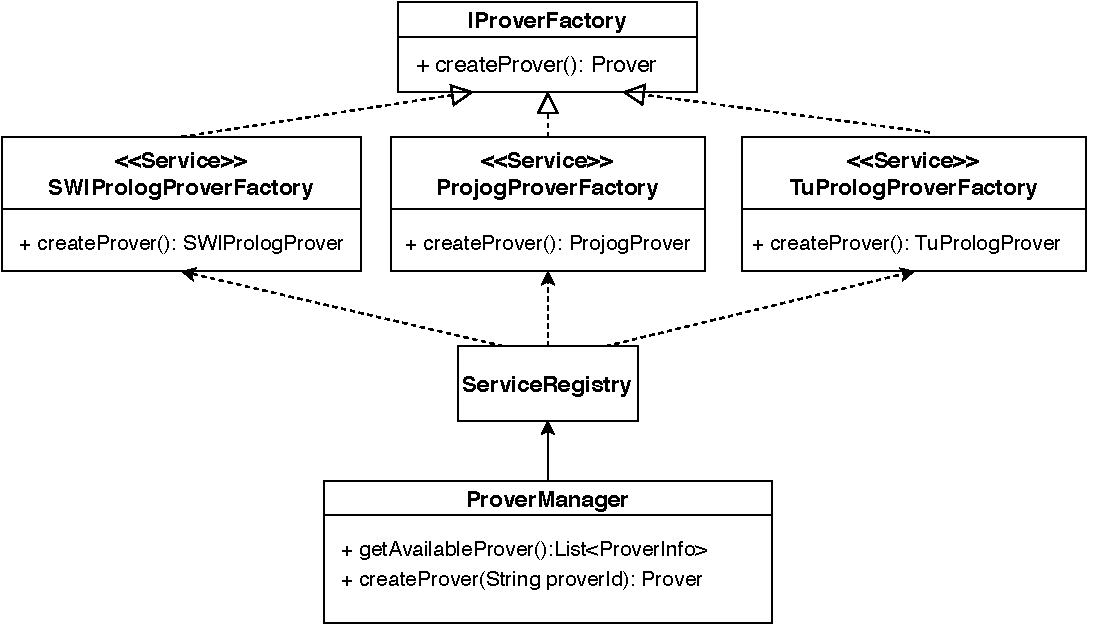
\includegraphics[width=1\textwidth]{osgi.pdf}
\end{figure}
\end{frame}

\end{document}
